% !TeX spellcheck = pl_PL
%%%%%%%%%%%%%%%%%%%%%%%%%%%%%%%%%%%%%%%%%%%
%                                        %
% Szablon pracy dyplomowej magisterskiej %
% zgodny  z aktualnymi  przepisami  SZJK %
%                                        %
%%%%%%%%%%%%%%%%%%%%%%%%%%%%%%%%%%%%%%%%%%
%                                        %
%  (c) Krzysztof Simiński, 2018-2023     %
%                                        %
%%%%%%%%%%%%%%%%%%%%%%%%%%%%%%%%%%%%%%%%%%
%                                        %
% Najnowsza wersja szablonów jest        %
% podstępna pod adresem                  %
% github.com/ksiminski/polsl-aei-theses  %
%                                        %
%%%%%%%%%%%%%%%%%%%%%%%%%%%%%%%%%%%%%%%%%%
%
%
% Projekt LaTeXowy zapewnia odpowiednie formatowanie pracy,
% zgodnie z wymaganiami Systemu zapewniania jakości kształcenia.
% Proszę nie zmieniać ustawień formatowania (np. fontu,
% marginesów, wytłuszczeń, kursywy itd. ).
%
% Projekt można kompilować na kilka sposobów.
%
% 1. kompilacja pdfLaTeX
%
% pdflatex main
% bibtex   main
% pdflatex main
% pdflatex main
%
%
% 2. kompilacja XeLaTeX
%
% Kompilatacja przy użyciu XeLaTeXa różni się tym, że na stronie
% tytułowej używany jest font Calibri. Wymaga to jego uprzedniego
% zainstalowania.
%
% xelatex main
% bibtex  main
% xelatex main
% xelatex main
%
%
%%%%%%%%%%%%%%%%%%%%%%%%%%%%%%%%%%%%%%%%%%%%%%%%%%%%%
% W przypadku pytań, uwag, proszę pisać na adres:   %
%      krzysztof.siminski(małpa)polsl.pl            %
%%%%%%%%%%%%%%%%%%%%%%%%%%%%%%%%%%%%%%%%%%%%%%%%%%%%%
%
% Chcemy ulepszać szablony LaTeXowe prac dyplomowych.
% Wypełniając ankietę spod poniższego adresu pomogą
% Państwo nam to zrobić. Ankieta jest całkowicie
% anonimowa. Dziękujemy!


% https://docs.google.com/forms/d/e/1FAIpQLScyllVxNKzKFHfILDfdbwC-jvT8YL0RSTFs-s27UGw9CKn-fQ/viewform?usp=sf_link
%
%%%%%%%%%%%%%%%%%%%%%%%%%%%%%%%%%%%%%%%%%%%%%%%%%%%%%%%%%%%%%%%%%%%%%%%%%

%%%%%%%%%%%%%%%%%%%%%%%%%%%%%%%%%%%%%%%%%%%%%%%
%                                             %
% PERSONALIZACJA PRACY – DANE PRACY           %
%                                             %
%%%%%%%%%%%%%%%%%%%%%%%%%%%%%%%%%%%%%%%%%%%%%%%

% Proszę wpisać swoje dane w poniższych definicjach.

% TODO
% dane autora
\newcommand{\FirstNameAuthor}{Mateusz}
\newcommand{\SurnameAuthor}{Marczewski}
\newcommand{\IdAuthor}{282700}   % numer albumu  (bez $\langle$ i $\rangle$)

% drugi autor:
%\newcommand{\FirstNameCoauthor}{Imię}   % Jeżeli jest drugi autor, to tutaj należy podać imię.
%\newcommand{\SurnameCoauthor}{Nazwisko} % Jeżeli jest drugi autor, to tutaj należy podać nazwisko.
%\newcommand{\IdCoauthor}{$\langle$wpisać właściwy$\rangle$}  % numer albumu drugiego autora (bez $\langle$ i $\rangle$)
% Gdy nie ma drugiego autora, należy zostawić poniższe definicje puste, jak poniżej. Gdy jest drugi autor, należy zakomentować te linie.
\newcommand{\FirstNameCoauthor}{} % Jeżeli praca ma tylko jednego autora, to dane drugiego autora zostają puste.
\newcommand{\SurnameCoauthor}{}   % Jeżeli praca ma tylko jednego autora, to dane drugiego autora zostają puste.
\newcommand{\IdCoauthor}{}  % Jeżeli praca ma tylko jednego autora, to dane drugiego autora zostają puste.
%%%%%%%%%%

\newcommand{\Supervisor}{Dr hab. inż. Arkadiusz Biernacki}     % dane promotora (bez $\langle$ i $\rangle$)
\newcommand{\Title}{Moduł do obsługi importów danych finansowych z plików PDF}           % tytuł pracy po polsku
\newcommand{\TitleAlt}{Module for importing inventory data from PDF files}                     % thesis title in English
\newcommand{\Program}{Informatyka}            % kierunek studiów  (bez $\langle$ i $\rangle$)
\newcommand{\Specialisation}{Internet i technologie sieciowe}     % specjalność  (bez $\langle$ i $\rangle$)
\newcommand{\Departament}{Sieci i Systemów Komputerowych}        % katedra promotora  (bez $\langle$ i $\rangle$)

% Jeżeli został wyznaczony promotor pomocniczy lub opiekun, proszę go/ją wpisać ...
\newcommand{\Consultant}{} % dane promotora pomocniczego, opiekuna (bez $\langle$ i $\rangle$)
% ... w przeciwnym razie proszę zostawić puste miejsce jak poniżej:
%\newcommand{\Consultant}{} % brak promotowa pomocniczego / opiekuna

% koniec fragmentu do modyfikacji
%%%%%%%%%%%%%%%%%%%%%%%%%%%%%%%%%%%%%%%%%%


%%%%%%%%%%%%%%%%%%%%%%%%%%%%%%%%%%%%%%%%%%%%%%%
%                                             %
% KONIEC PERSONALIZACJI PRACY                 %
%                                             %
%%%%%%%%%%%%%%%%%%%%%%%%%%%%%%%%%%%%%%%%%%%%%%%

%%%%%%%%%%%%%%%%%%%%%%%%%%%%%%%%%%%%%%%%


%%%%%%%%%%%%%%%%%%%%%%%%%%%%%%%%%%%%%%%%%%%%%%%
%                                             %
% PROSZĘ NIE MODYFIKOWAĆ PONIŻSZYCH USTAWIEŃ! %
%                                             %
%%%%%%%%%%%%%%%%%%%%%%%%%%%%%%%%%%%%%%%%%%%%%%%



\documentclass[a4paper,twoside,12pt]{book}
\usepackage[utf8]{inputenc}                                      
\usepackage[T1]{fontenc}  
\usepackage{amsmath,amsfonts,amssymb,amsthm}
\usepackage[british,polish]{babel} 
\usepackage{indentfirst}
\usepackage{xurl}
\usepackage{xstring}
\usepackage{ifthen}



\usepackage{ifxetex}

\ifxetex
	\usepackage{fontspec}
	\defaultfontfeatures{Mapping=tex—text} % to support TeX conventions like ``——-''
	\usepackage{xunicode} % Unicode support for LaTeX character names (accents, European chars, etc)
	\usepackage{xltxtra} % Extra customizations for XeLaTeX
\else
	\usepackage{lmodern}
\fi



\usepackage[margin=2.5cm]{geometry}
\usepackage{graphicx} 
\usepackage{hyperref}
\usepackage{booktabs}
\usepackage{tikz}
\usepackage{pgfplots}
\usepackage{mathtools}
\usepackage{geometry}
\usepackage{subcaption}   % subfigures
\usepackage[page]{appendix} % toc,
\renewcommand{\appendixtocname}{Dodatki}
\renewcommand{\appendixpagename}{Dodatki}
\renewcommand{\appendixname}{Dodatek}

\usepackage{csquotes}
\usepackage[natbib=true,backend=bibtex,maxbibnames=99]{biblatex}  % kompilacja bibliografii BibTeXem
%\usepackage[natbib=true,backend=biber,maxbibnames=99]{biblatex}  % kompilacja bibliografii Biberem
\bibliography{biblio}

\usepackage{ifmtarg}   % empty commands  

\usepackage{setspace}
\onehalfspacing


\frenchspacing



%%%% TODO LIST GENERATOR %%%%%%%%%

\usepackage{color}
\definecolor{brickred}      {cmyk}{0   , 0.89, 0.94, 0.28}

\makeatletter \newcommand \kslistofremarks{\section*{Uwagi} \@starttoc{rks}}
  \newcommand\l@uwagas[2]
    {\par\noindent \textbf{#2:} %\parbox{10cm}
{#1}\par} \makeatother


\newcommand{\ksremark}[1]{%
{%\marginpar{\textdbend}
{\color{brickred}{[#1]}}}%
\addcontentsline{rks}{uwagas}{\protect{#1}}%
}

\newcommand{\comma}{\ksremark{przecinek}}
\newcommand{\nocomma}{\ksremark{bez przecinka}}
\newcommand{\styl}{\ksremark{styl}}
\newcommand{\ortografia}{\ksremark{ortografia}}
\newcommand{\fleksja}{\ksremark{fleksja}}
\newcommand{\pauza}{\ksremark{pauza `--', nie dywiz `-'}}
\newcommand{\kolokwializm}{\ksremark{kolokwializm}}
\newcommand{\cudzyslowy}{\ksremark{,,polskie cudzysłowy''}}

%%%%%%%%%%%%%% END OF TODO LIST GENERATOR %%%%%%%%%%%

\newcommand{\printCoauthor}{%		
    \StrLen{\FirstNameCoauthor}[\FNCoALen]
    \ifthenelse{\FNCoALen > 0}%
    {%
		{\large\bfseries\Coauthor\par}
	
		{\normalsize\bfseries \LeftId: \IdCoauthor\par}
    }%
    {}
} 

%%%%%%%%%%%%%%%%%%%%%
\newcommand{\autor}{%		
    \StrLen{\FirstNameCoauthor}[\FNCoALenXX]
    \ifthenelse{\FNCoALenXX > 0}%
    {\FirstNameAuthor\ \SurnameAuthor, \FirstNameCoauthor\ \SurnameCoauthor}%
	{\FirstNameAuthor\ \SurnameAuthor}%
}
%%%%%%%%%%%%%%%%%%%%%

\StrLen{\FirstNameCoauthor}[\FNCoALen]
\ifthenelse{\FNCoALen > 0}%
{%
\author{\FirstNameAuthor\ \SurnameAuthor, \FirstNameCoauthor\ \SurnameCoauthor}
}%
{%
\author{\FirstNameAuthor\ \SurnameAuthor}
}%

%%%%%%%%%%%% ZYWA PAGINA %%%%%%%%%%%%%%%
% brak kapitalizacji zywej paginy
\usepackage{fancyhdr}
\pagestyle{fancy}
\fancyhf{}
\fancyhead[LO]{\nouppercase{\it\rightmark}}
\fancyhead[RE]{\nouppercase{\it\leftmark}}
\fancyhead[LE,RO]{\it\thepage}


\fancypagestyle{tylkoNumeryStron}{%
   \fancyhf{} 
   \fancyhead[LE,RO]{\it\thepage}
}

\fancypagestyle{bezNumeracji}{%
   \fancyhf{} 
   \fancyhead[LE,RO]{}
}


\fancypagestyle{NumeryStronNazwyRozdzialow}{%
   \fancyhf{} 
   \fancyhead[LE]{\nouppercase{\autor}}
   \fancyhead[RO]{\nouppercase{\leftmark}} 
   \fancyfoot[CE, CO]{\thepage}
}


%%%%%%%%%%%%% OBCE WTRETY  
\newcommand{\obcy}[1]{\emph{#1}}
\newcommand{\english}[1]{{\selectlanguage{british}\obcy{#1}}}
%%%%%%%%%%%%%%%%%%%%%%%%%%%%%

% polskie oznaczenia funkcji matematycznych
\renewcommand{\tan}{\operatorname {tg}}
\renewcommand{\log}{\operatorname {lg}}

% jeszcze jakies drobiazgi

\newcounter{stronyPozaNumeracja}

%%%%%%%%%%%%%%%%%%%%%%%%%%% 
\newcommand{\printOpiekun}[1]{%		

    \StrLen{\Consultant}[\mystringlen]
    \ifthenelse{\mystringlen > 0}%
    {%
       {\large{\bfseries OPIEKUN, PROMOTOR POMOCNICZY}\par}
       
       {\large{\bfseries \Consultant}\par}
    }%
    {}
} 
%
%%%%%%%%%%%%%%%%%%%%%%%%%%%%%%%%%%%%%%%%%%%%%%
 
% Proszę nie modyfikować poniższych definicji!
\newcommand{\Author}{\FirstNameAuthor\ \MakeUppercase{\SurnameAuthor}} 
\newcommand{\Coauthor}{\FirstNameCoauthor\ \MakeUppercase{\SurnameCoauthor}}
\newcommand{\Type}{PRACA MAGISTERSKA}
\newcommand{\Faculty}{Wydział Automatyki, Elektroniki i Informatyki} 
\newcommand{\Polsl}{Politechnika Śląska}
\newcommand{\Logo}{politechnika_sl_logo_bw_pion_pl.pdf}
\newcommand{\LeftId}{Nr albumu}
\newcommand{\LeftProgram}{Kierunek}
\newcommand{\LeftSpecialisation}{Specjalność}
\newcommand{\LeftSUPERVISOR}{PROWADZĄCY PRACĘ}
\newcommand{\LeftDEPARTMENT}{KATEDRA}
%%%%%%%%%%%%%%%%%%%%%%%%%%%%%%%%%%%%%%%%%%%%%%

%%%%%%%%%%%%%%%%%%%%%%%%%%%%%%%%%%%%%%%%%%%%%%%
%                                             %
% KONIEC USTAWIEŃ                             %
%                                             %
%%%%%%%%%%%%%%%%%%%%%%%%%%%%%%%%%%%%%%%%%%%%%%%




%%%%%%%%%%%%%%%%%%%%%%%%%%%%%%%%%%%%%%%%%%%%%%%
%                                             %
% MOJE PAKIETY, USTAWIENIA ITD                %
%                                             %
%%%%%%%%%%%%%%%%%%%%%%%%%%%%%%%%%%%%%%%%%%%%%%%

% Tutaj proszę umieszczać swoje pakiety, makra, ustawienia itd.


 
%%%%%%%%%%%%%%%%%%%%%%%%%%%%%%%%%%%%%%%%%%%%%%%%%%%%%%%%%%%%%%%%%%%%%
% listingi i fragmentu kodu źródłowego 
% pakiet: listings lub minted
% % % % % % % % % % % % % % % % % % % % % % % % % % % % % % % % % % % 

% biblioteka listings
\usepackage{listings}
\lstset{%
morekeywords={string,exception,std,vector},% słowa kluczowe rozpoznawane przez pakiet listings
language=C++,% C, Matlab, Python, SQL, TeX, XML, bash, ... – vide https://www.ctan.org/pkg/listings
commentstyle=\textit,%
identifierstyle=\textsf,%
keywordstyle=\sffamily\bfseries, %\texttt, %
%captionpos=b,%
tabsize=3,%
frame=lines,%
numbers=left,%
numberstyle=\tiny,%
numbersep=5pt,%
breaklines=true,%
escapeinside={@*}{*@},%
}

% % % % % % % % % % % % % % % % % % % % % % % % % % % % % % % % % % % 
% pakiet minted
%\usepackage{minted}

% pakiet wymaga specjalnego kompilowania:
% pdflatex -shell-escape main.tex
% xelatex  -shell-escape main.tex

%\usepackage[chapter]{minted} % [section]
%%\usemintedstyle{bw}   % czarno-białe kody 
%
%\setminted % https://ctan.org/pkg/minted
%{
%%fontsize=\normalsize,%\footnotesize,
%%captionpos=b,%
%tabsize=3,%
%frame=lines,%
%framesep=2mm,
%numbers=left,%
%numbersep=5pt,%
%breaklines=true,%
%escapeinside=@@,%
%}

%%%%%%%%%%%%%%%%%%%%%%%%%%%%%%%%%%%%%%%%%%%%%%%%%%%%%%%%%%%%%%%%%%%%%



%%%%%%%%%%%%%%%%%%%%%%%%%%%%%%%%%%%%%%%%%%%%%%%
%                                             %
% KONIEC MOICH USTAWIEŃ                       %
%                                             %
%%%%%%%%%%%%%%%%%%%%%%%%%%%%%%%%%%%%%%%%%%%%%%%



%%%%%%%%%%%%%%%%%%%%%%%%%%%%%%%%%%%%%%%%


\begin{document}
%\kslistofremarks

\frontmatter

%%%%%%%%%%%%%%%%%%%%%%%%%%%%%%%%%%%%%%%%%%%%%%%
%                                             %
% PROSZĘ NIE MODYFIKOWAĆ STRONY TYTUŁOWEJ!    %
%                                             %
%%%%%%%%%%%%%%%%%%%%%%%%%%%%%%%%%%%%%%%%%%%%%%%


%%%%%%%%%%%%%%%%%%  STRONA TYTUŁOWA %%%%%%%%%%%%%%%%%%%
\pagestyle{empty}
{
	\newgeometry{top=1.5cm,%
	             bottom=2.5cm,%
	             left=3cm,
	             right=2.5cm}
 
	\ifxetex 
	  \begingroup
	  \setsansfont{Calibri}
	   
	\fi 
	 \sffamily
	\begin{center}
	\includegraphics[width=50mm]{\Logo}
	 
	
	{\Large\bfseries\Type\par}
	
	\vfill  \vfill  
			 
	{\large\Title\par}
	
	\vfill  
		
	{\large\bfseries\Author\par}
	
	{\normalsize\bfseries \LeftId: \IdAuthor}

	\printCoauthor
	
	\vfill  		
 
	{\large{\bfseries \LeftProgram:} \Program\par} 
	
	{\large{\bfseries \LeftSpecialisation:} \Specialisation\par} 
	 		
	\vfill  \vfill 	\vfill 	\vfill 	\vfill 	\vfill 	\vfill  
	 
	{\large{\bfseries \LeftSUPERVISOR}\par}
	
	{\large{\bfseries \Supervisor}\par}
				
	{\large{\bfseries \LeftDEPARTMENT\ \Departament} \par}
		
	{\large{\bfseries \Faculty}\par}
		
	\vfill  \vfill  

    	
    \printOpiekun{\Consultant}
    
	\vfill  \vfill  
		
    {\large\bfseries  Gliwice \the\year}

   \end{center}	
       \ifxetex 
       	  \endgroup
       \fi
	\restoregeometry
}
  
%%%%%%%%%%%%%%%%%%%%%%%%%%%%%%%%%%%%%%%%%%%%%%%
%                                             %
% KONIEC STRONY TYTUŁOWEJ                     %
%                                             %
%%%%%%%%%%%%%%%%%%%%%%%%%%%%%%%%%%%%%%%%%%%%%%%  


\cleardoublepage

\rmfamily\normalfont
\pagestyle{empty}


%%% No to zaczynamy pisać pracę :-) %%%%

% TODO
\subsubsection*{Tytuł pracy} 
\Title

\subsubsection*{Streszczenie}  
Głównym celem tego projektu jest opracowanie praktycznego oprogramowania, które automatyzuje proces wydobycia istotnych danych z tabel zawartych w dokumentach o formacie \emph{PDF} (Portable Document Format). Wybór formatu \emph{PDF} jako głównego celu wynika z jego szerokiego zastosowania i dostępności licznych zbiorów danych prezentowanych w danym typie plików. 

\subsubsection*{Słowa kluczowe} 
PDF, ekstrakcja danych, Adobe, wykrywanie tabel, ekstrakcja tabel
\subsubsection*{Thesis title} 
\begin{otherlanguage}{british}
\TitleAlt
\end{otherlanguage}

\subsubsection*{Abstract} 
\begin{otherlanguage}{british}
The main goal of this project is to develop practical software that automates the process of extracting relevant data from tables contained within documents in \emph{PDF} (Portable Document Format) format. The choice of the \emph{PDF} format as the primary target stems from its wide usage and the availability of numerous datasets presented in this file type.
\end{otherlanguage}
\subsubsection*{Key words}  
\begin{otherlanguage}{british}
 PDF, data extraction, Adobe, table detection, table extraction
\end{otherlanguage}




%%%%%%%%%%%%%%%%%% SPIS TRESCI %%%%%%%%%%%%%%%%%%%%%%
% Add \thispagestyle{empty} to the toc file (main.toc), because \pagestyle{empty} doesn't work if the TOC has multiple pages
\addtocontents{toc}{\protect\thispagestyle{empty}}
\tableofcontents

%%%%%%%%%%%%%%%%%%%%%%%%%%%%%%%%%%%%%%%%%%%%%%%%%%%%%
\setcounter{stronyPozaNumeracja}{\value{page}}
\mainmatter
\pagestyle{empty}

\cleardoublepage

\pagestyle{NumeryStronNazwyRozdzialow}

%%%%%%%%%%%%%% wlasciwa tresc pracy %%%%%%%%%%%%%%%%%

% TODO
\chapter{Wstęp}

%\begine}
%\end{itemize}

\section{Wprowadzenie w zagadnienie}

Importowanie danych z różnych źródeł, takich jak faktury zamówień, potwierdzenia sprzedaży, dane o załadunkach i tym podobne, a następnie importowanie ich do firmowych baz danych, jest problemem, nad którym chce się pochylić niniejsza praca. Jako sposób prezentacji takich danych często używane są tabele, jest to intuicyjny i bardzo efektywny sposób zapisu dużych zbiorów danych. Jest to metoda stosowana niezależnie od tego jaki typ danych chcemy przedstawić, z tego powodu nie ma żadnego standardu określającego jak takie tabele powinny być przedstawiane. Często różnią się one w zależności od celu i preferencji twórcy, jednak w obecnych czasach cyfryzacji, zazwyczaj  będą one również dostępne w formie plików \emph{PDF} (Portable Document Format), lub będzie możliwe ich do tej postaci zeskanowanie. Znacznie ułatwia to ich przechowywanie i podgląd, jednak utrudnia ekstrakcje danych z takich plików. 

W celu rozwiązania tego problemu, wiele firm wykorzystuje specjalnie przygotowane aplikacje, które pozwalają na automatyzację procesu importowania danych z plików \emph{PDF}. Takie aplikacje mogą importować dane w postaci plików \emph{PDF}, a następnie wykrywać w nich najważniejsze dane i eksportować je do żądanego formatu, obsługiwanego przez bazę danych lub inne aplikacje służące do zarządzania danymi. Takie aplikacje mogą przechowywać dane w własnym formacie, i pozwalać na łatwy dostęp do zasobów firmy, nawet bez znajomości działania baz danych. 

%\item osadzenie problemu w dziedzinie 
\section{Cel pracy}

Celem tej pracy jest utworzenie własnej aplikacji, która umożliwi łatwe wyeksportowanie danych z tabel znajdujących się w plikach o rozszerzeniu \emph{PDF}, do łatwiej obsługiwanych plików wyjściowych w formacie \emph{CSV} (comma-separated values). Aplikacja zostanie stworzona w taki sposób, aby umożliwiała samodzielne użytkowanie programu bezpośrednio z dokumentami PDF, a także wykorzystywanie jej jako część innych narzędzi i projektów. Wyjście stworzonej aplikacji oprogramowania ma umożliwić łatwą, dalszą obsługę wyeksportowanych danych, dlatego zdecydowano się wykorzystać wyżej wspomniany format CSV. Cały kod źródłowy tego projektu pracy dyplomowej zostanie udostępniony online na platformie www.github.com

\section{Budowa Tabeli}

Jednym z częściej spotykanych modeli koncepcyjnych tabeli jest ten zaproponowany przez Wanga \cite{bib:Wang}, a później rozbudowany przez Hursta \cite{Hurst}. Wang definiuje tabelę jako podzieloną na cztery główne obszary: 
\begin{itemize}
\item the stub czyli pień, jest to 
kolumna, która zawiera nagłówki wierszy i podnagłówki; 
\item boxhead tworzący pojemnik na nagłówki kolumn (z wyłączeniem nagłówka kolumny) 
\item stubhead, nagłówek pierwszej kolumny, który zawiera nagłówek dla kolumny, 
\item body czyli główną treść tabeli, część ta zawiera faktyczne dane tabeli. 
\end{itemize}
W niniejszej pracy magisterskiej definicje Wanga zostały nieco dostosowane, tak aby nagłówek kolumny był uważany za część kolumny. Warto wspomnieć, że oczywiście nie każda tabela jest tak samo zbudowana. Na przykład, dla dużej liczby tabel, nagłówki kolumn nie są zebrane w jednej ramce. Oprócz tych definicji, praca magisterska korzysta z definicji takich elementów tabeli jak: nagłówek, kolumna, wiersz, komórka. Rysunek 1.1 ilustruje te definicje.

\begin{figure}
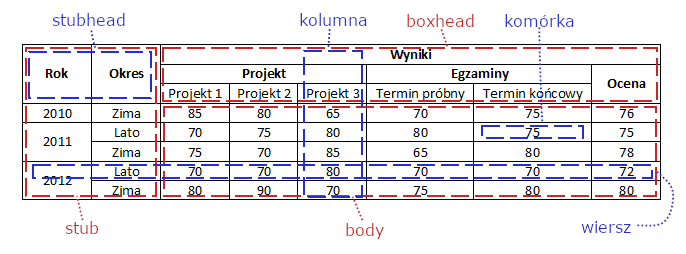
\includegraphics[width=1\textwidth]{./images/table.png}
\caption{Budowa tebeli z wyszczególnieniem omówionych elementów}
\label{fig:pdf_logo}
\end{figure}

%\item zakres pracy 
\section{Charakterystyka rozdziałów}

W niniejszej pracy naukowej przedstawiamy szereg rozdziałów, które składają się na kompleksową analizę modułu do importowania danych inwentaryzacyjnych z plików \emph{PDF}. Każdy z tych rozdziałów ma swoje unikalne znaczenie i koncentruje się na konkretnych aspektach badania. Poniżej przedstawiamy krótką charakterystykę poszczególnych rozdziałów:

Rozdział 2: Definiowanie wymagań

W tym rozdziale skupiamy się na ustaleniu konkretnych wymagań dla modułu lub biblioteki służącej do importowania danych z plików \emph{PDF}.
Analizujemy różne typy danych, które mają zostać zaimportowane, oraz identyfikujemy pola w plikach \emph{PDF}, które będą przechwytywane.
Przeanalizujemy również inne formaty plików, z którymi moduł będzie pracował, aby zapewnić wszechstronność i elastyczność rozwiązania.

Rozdział 3: Badanie istniejących rozwiązań

W tym rozdziale skoncentrujemy się na dokładnym przejrzeniu istniejących modułów i bibliotek dostępnych na rynku do importowania danych z plików \emph{PDF}.
Przeanalizujemy funkcje, jakie oferują te rozwiązania oraz przetestujemy ich możliwości. Celem tego rozdziału jest zgłębienie istniejących rozwiązań i dostrzeżenie ich mocnych i słabych stron w celu stworzenia solidnej podstawy do dalszych badań.

Rozdział 4: Ocena dostępnych opcji

W tym rozdziale przeprowadzimy szczegółową ocenę dostępnych opcji na podstawie wcześniej zdefiniowanych wymagań. Porównamy różne rozwiązania pod kątem ich zgodności z określonymi wymaganiami, aby wybrać najlepszą opcję dla dalszych badań i implementacji. Porównane zostaną również nasza opinia oraz opinie i oceny dostępne w artykułach naukowych, w celu poprawnej analizy rozwiązania.

Rozdział 5: Rozwój istniejących rozwiązań

W tym rozdziale skupimy się na rozwoju istniejących rozwiązań, takich jak dostosowanie ich do specyficznych potrzeb  projektu. Przeanalizujemy również wymagane zasoby i umiejętności potrzebne do kontynuacji rozwoju i utrzymania modułu opartego na danej bibliotece.

Rozdział 6: Rozwój własnego rozwiązania

Ten rozdział koncentruje się na własnym rozwiązaniu, uwzględniając wyniki poprzednich analiz i badań. Przeanalizujemy wyniki, które udało się osiągnąć przy wykorzystaniu własnego rozwiązania i porównamy je z istniejącymi na rynku.

Rozdział 7: Dokumentacja i udostępnianie wybranego rozwiązania

W tym rozdziale omówimy proces tworzenia dokumentacji dla wybranego rozwiązania, aby umożliwić innym użytkownikom skorzystanie z modułu. Przeanalizujemy również możliwość udostępnienia rozwiązania jako projektu open-source dla społeczności programistycznej.

Rozdział 8: Podsumowanie

W ostatnim rozdziale dokonamy podsumowania całego badania, podkreślając najważniejsze wnioski i rezultaty. Przedstawimy również implikacje wynikające z naszej pracy badawczej oraz sugestie dotyczące przyszłych kierunków rozwoju i badań w tej dziedzinie.

Każdy z tych rozdziałów przyczynia się do pełnego zrozumienia problemu i tworzy spójną strukturę pracy badawczej dotyczącej modułu do importowania danych inwentaryzacyjnych z plików PDF.


% TODO
\chapter{Definiowanie wymagań}  % Analiza tematu
% 

%\begin{itemize}
%\end{itemize}
\section{Formaty plików występujące w pracy}

W tym miejscu opisane zostaną formaty plików, z których korzystano podczas tworzenia te pracy, to jest, \emph{PDF} oraz \emph{CSV}. 

\subsection{Pliki PDF}

Format \emph{PDF} (Portable Document Format) jest zbudowany zgodnie z określonymi specyfikacjami opracowanymi przez firmę Adobe Systems na początku lat 90. Format ten ma na celu zapewnienie niezależności od platformy i zachowanie spójności formatowania, niezależnie od urządzenia, na którym jest wyświetlany\cite{bib:pdf_ref}. Specyfikacja \emph{PDF} została udostępniona bezpłatnie w 1993 roku, ale pozostała jako format własnościowy, aż w 2008 roku została oficjalnie wydana jako otwarty standard (ISO 32000-1:2008)\cite{bib:iso} Ta licencja przyznaje bezpłatne prawa licencyjne do wszystkich patentów należących do Adobe, które są niezbędne do tworzenia, używania, sprzedaży i dystrybucji implementacji zgodnych z formatem \emph{PDF} \cite{bib:adobe_cert}. Oprócz tych cech, pliki \emph{PDF} oferują dobrą kompresję, zmniejszając rozmiar pliku i czyniąc format idealnym do dystrybucji online. Logo Adobe PDF jest pokazane na Rys. \ref{fig:pdf_logo}.

\begin{figure}
\centering

\includegraphics[width=0.2\textwidth]{./images/PDF_logo.png}
\caption{Logo formatu PDF firmy Adobe jest rozpoznawalne dla wielu osób ze względu na popularność 
\cite{bib:pdf_logo}}
\label{fig:pdf_logo}
\end{figure}

W pierwszej kolejności warto zwrócić uwagę na różnice między starszymi a nowszymi wersjami formatu \emph{PDF}. Pliki \emph{PDF} są stale rozwijane i udoskonalane, dlatego ważne jest, aby zrozumieć, jakie funkcje i możliwości są dostępne w różnych wersjach. Niektóre starsze wersje mogą nie obsługiwać niektórych zaawansowanych funkcji, co należy wziąć pod uwagę przy tworzeniu modułu importującego.

Kolejnym aspektem jest analiza możliwości skryptowania i interaktywności w plikach \emph{PDF}. Niektóre pliki \emph{PDF} mogą zawierać skrypty JavaScript lub elementy interaktywne, takie jak formularze, przyciski, linki itp. Istotne jest zrozumienie tych elementów i określenie, czy i w jaki sposób można je obsłużyć podczas importowania danych.

Dodatkowo, badamy w tym typie dokumentów wykorzystuje się różne technologie i standardy związane z potrzebami użytkownika. Są nimi standardy takie jak PDF/A (standard archiwizacji), PDF/X (standard dla publikacji drukowanych) czy PDF/UA (standard dostępności). W zależności od specyfiki aplikacji i wymagań postawionych przed rozwiązaniem, konieczne może być uwzględnienie tych standardów i zapewnienie zgodności modułu importującego.

Plik \emph{PDF} składa się z różnych elementów i struktur, które razem tworzą dokument. Jego strukturę możemy podzielić na 4 części: 
\begin{itemize}
\item Header - informacje o strukturze i metadanych pliku \emph{PDF}, takich jak wersja specyfikacji \emph{PDF}, typ pliku, używane czcionki, rozmiar strony itp.
\item Body - treść dokumentu, taką jak tekst, obrazy, grafiki, tabele itp. Ciało składa się z sekwencji obiektów PDF, które są odpowiedzialne za przechowywanie danych i struktury dokumentu.
\item Xref table - spis wszystkich obiektów, używanych w dokumencie. Każdy obiekt ma unikalny numer identyfikacyjny i jest przechowywany w formacie klucz-wartość.
\item Trailer - informacje o lokalizacji i numerze generacji wszystkich obiektów w pliku \emph{PDF}. Jest to wykorzystywane do odnalezienia i odzyskania obiektów podczas odczytu lub modyfikacji pliku.
\end{itemize}

Trudność przy obsłudze plików typu \emph{PDF} jest zauważalna przy przeanalizowaniu tej struktury. Zazwyczaj pliki te odczytuje się od końca, wynika to z tego, że na końcu zawarte są informacje o wersji zapisu, oraz położeniu najważniejszych struktur.

Analiza formatów plików \emph{PDF} pozwala nam lepiej zrozumieć złożoność i różnorodność plików, które będą importowane do tworzonej aplikacji. Pozwala to na dokładne określenie wymagań tworzonego modułu i odpowiednie dostosowanie go do różnych formatów plików \emph{PDF}, które będzie obsługiwać.

\subsection{Pliki CSV}

W pliku \emph{CSV} dane są przechowywane w formie tabeli, gdzie każdy wiersz reprezentuje rekord, a poszczególne pola w rekordzie są oddzielane separatorem, najczęściej przecinkiem, jak sugeruje sama nazwa tego formatu, jednak inne separatory, takie jak średnik, również są stosowane w poszczególnych przypadkach. Pliki \emph{CSV} wyróżnia to, że mimo możliwości przechowywania złożonych tabel z danymi, jest on formatem tekstowym. Oznacza to, że dane są zapisywane jako tekst, bez złożonej struktury danych, a dopiero następnie można je wyświetlać w postaci tabel lub arkuszy. Można w nich przechowywać dzięki temu różne rodzaje danych, takie jak tekst, liczby, daty itp. bez znacznego zwiększenia ich objętości pamięciowej. Wyżej wspomniane wariacje w postaci wykorzystanych separatorów, pozwalają na zawieranie dowolnych znaków specjalnych, takich jak przecinki w danych liczbowych.

\section{Przegląd typów danych do importowania}

Plik \emph{PDF} może zawierać różne formy zapisu informacji, takie jak tekst, tabele, obrazy, formularze itp. W celu efektywnego importowania danych z tych plików do innego formatu, konieczne jest zidentyfikowanie i zrozumienie charakterystyki tych typów danych. 

Przede wszystkim, analizujemy sposoby ekstrakcji tekstu z plików \emph{PDF}. Tekst może występować zarówno w postaci prostej, takiej jak  akapity, nagłówki lub stopki. Jednak często występuje również w bardziej złożonej postaci np. listy, tabele.

Kolejnym istotnym typem danych są tabele. Pliki \emph{PDF}, które będziemy analizować zawierają tabele z danymi, które muszą być zaimportowane do innego formatu w taki sposób, aby zachować strukturę tabelaryczną. Celem tej pracy jest przedstawienie metody identyfikacji tabel oraz ekstrakcji danych z nich, co zostanie uczynione w kolejnych rozdziałach. Tabele jakie mogą występować w plikach \emph{PDF} to zarówno prostsze zbiory danych bez łączeń komórek, jak i bardziej zaawansowane struktury tabelaryczne, różnią się one przede wszystkim położeniem komórek. Nie wszystkie komórki muszą zawierać opis jaki typ danych jest w nich zapisany, dodatkowo zapis ten może być niespójny jeżeli tabela byłaby uzupełniana przez innych pracowników.

W plikach \emph{PDF} mogą również występować obrazy, formularze, lub inne struktury, które są zapisane w części Xref pliku \emph{PDF}, przez co możemy je łatwo ominąć podczas ekstrakcji tabeli.

Przegląd typów danych do importowania umożliwia nam lepsze zrozumienie różnorodności informacji zawartych w plikach \emph{PDF} oraz wyznaczenie kierunku dalszych badań i rozwoju modułu importującego.

% TODO

\section{Problemy związane z importowaniem danych}

Cały proces ekstrakcji danych opiera się na wcześniejszym zdefiniowaniu informacji, na których będą operować algorytmy. Biblioteka o nazwie pdfminer\cite{bib:pdfminer} została wykorzystana w celu ekstrakcji tekstu z plików \emph{PDF}, a algorytmy wykorzystane w projekcie, przetwarzają i interpretują informacje o składnikach pliku i w wypadku potrzeby wyeksportowania tekstu, przekazują je do podanej biblioteki. Dostępne dane nie są tak szczegółowe, jak by się mogło wydawać. Na przykład, dany blok zawierający słowo nie ma dostępnych informacji o użytej czcionce ani stylu czcionki. Podczas wyodrębniania tekstu z pliku \emph{PDF}, proces wyodrębniania zazwyczaj traktuje cały tekst jako znajdujący się na tym samym poziomie linii bazowej.  

Tekst w dokumencie \emph{PDF} jest otrzymywany dla każdej pojedynczej strony w postaci prostokątnych obszarów zawierających pojedyncze słowo tekstu. Każdy prostokątny obszar elementu jest zdefiniowany za pomocą współrzędnych, co nadaje mu dokładne i jednoznaczne położenie oraz rozmiar (szerokość i wysokość) na stronie. Boki pudełek tekstowych zawsze są wyrównane do krawędzi stron; innymi słowy, nie ma przechylonych ani skośnych prostokątów. Formatowanie tekstu takie jak tekst w postaci indeksu górnego lub dolnego, wykorzystane czcionki, pogrubienia, pochylenia itp. zazwyczaj osiąga się poprzez metryki czcionek i dostosowania pozycji, a nie poprzez wyraźne znaczniki.

Ponadto, nie ma żadnych informacji na temat tego, czy dane słowa są częściami zdania, tabeli czy innej struktury. Asocjacja słów i tworzenie zdań (oraz komórek tabeli) musi być wykonane przez algorytmy ekstrakcji danych poprzez analizowanie i przetwarzanie elementów na stronie. Jeśli słowo jest rozdzielone myślnikiem na końcu linii i kontynuuje na kolejnej, jest ono podzielone na dwie zupełnie niepowiązane ramki tekstu.

Współrzędne ramek tekstu są zapisywane za pomocą punktów. W formacie \emph{PDF} punkt to typograficzna jednostka miary, która jest definiowana jako 1/72 cala. Ta spójna jednostka jest wykorzystywana w plikach \emph{PDF} do pozycjonowania i określania nie tylko pozycji i rozmiaru tekstu ale również innych elementów, w tym obrazów i tabel. Użycie punktów jako jednostki pomiarowej w plikach \emph{PDF} zapewnia spójność układu i wizualnego wyglądu treści bez względu na urządzenie wyświetlające lub drukujące. Poniżej znajduje się przeliczenie rozmiaru punktu z cali na milimetry

\begin{align}
punkt = \frac{1}{72} cala = \frac{25.4}{72} mm = 0.3527(7) mm
\end{align}

Z tego powodu cały proces ekstrakcji danych z tabel znajdujących się w plikach \emph{PDF}, można podzielić na mniejsze indywidualne zadania

\begin{enumerate}
\item Odczytywanie zawartości pliku \emph{PDF}.
\item Rozpoznawanie linii separatorów i siatek.
\item Lokalizowanie obszarów z tabelami w dokumencie.
\item Określanie struktury wierszy i kolumn tabeli.
\item Określanie wierszy nagłówków tabeli.
\item Formatowanie i importowanie danych z tabeli do aplikacji w języku Python.
\item Eksportowanie tabeli do pliku o formacie \emph{CSV}.
\end{enumerate}

Dzięki przeprowadzeniu z powodzeniem wyżej wymienionych kroków, uzyskamy pożądany efekt, którym jest tabela w edytowalnym formacie zapisana w osobnym pliku.

\chapter{Algorytmy}

\section{Odczytywanie zawartości pliku \emph{PDF}}
\section{Rozpoznawanie linii separatorów i siatek}
\section{Lokalizowanie obszarów z tabelami w dokumencie}
\section{Określanie struktury wierszy i kolumn tabeli}
\section{Określanie wierszy nagłówków tabeli}
\section{Formatowanie i importowanie danych z tabeli do aplikacji w języku Python}
\section{Eksportowanie tabeli do pliku o formacie \emph{CSV}}

\chapter{Badanie istniejących rozwiązań} 

tekst

\section{Przegląd istniejących modułów i bibliotek do importowania danych z PDF}

\section{Funkcje istniejących rozwiązań}

\section{Oceny użytkowników i opinie na temat istniejących rozwiązań}

W całym dokumencie powinny znajdować się odniesienia do zawartych w nim ilustracji (rys. \ref{fig:2}).

\begin{figure}
\centering
\begin{tikzpicture}
\begin{axis}[
    y tick label style={
        /pgf/number format/.cd,
            fixed,   % po zakomentowaniu os rzednych jest indeksowana wykladniczo
            fixed zerofill, % 1.0 zamiast 1
            precision=1,
        /tikz/.cd
    },
    x tick label style={
        /pgf/number format/.cd,
            fixed,
            fixed zerofill,
            precision=2,
        /tikz/.cd
    }
]
\addplot [domain=0.0:0.1] {rnd};
\end{axis} 
\end{tikzpicture}
\caption{Wykres przebiegu funkcji.} % Podpis jest zawsze POD rysunkiem.
\label{fig:2}
\end{figure}


%%%%%%%%%%%%%%%%%%%%%
%% RYSUNEK Z PLIKU
%
%\begin{figure}
%\centering
%
\includegraphics[width=0.5\textwidth]{./politechnika_sl_logo_bw_pion_pl.pdf}
%\caption{Podpis rysunku zawsze pod rysunkiem.}
%\label{fig:etykieta-rysunku}
%\end{figure}
%Rys. \ref{fig:etykieta-rysunku} przestawia …
%%%%%%%%%%%%%%%%%%%%%
%
%%%%%%%%%%%%%%%%%%%%%
%% WIELE RYSUNKÓW 
%
%\begin{figure}
%\centering
%\begin{subfigure}{0.4\textwidth}
%    
\includegraphics[width=\textwidth]{./politechnika_sl_logo_bw_pion_pl.pdf}
%    \caption{Lewy górny rysunek.}
%    \label{fig:lewy-gorny}
%\end{subfigure}
%\hfill
%\begin{subfigure}{0.4\textwidth}
%    
\includegraphics[width=\textwidth]{./politechnika_sl_logo_bw_pion_pl.pdf}
%    \caption{Prawy górny rysunek.}
%    \label{fig:prawy-gorny}
%\end{subfigure}
%
%\begin{subfigure}{0.4\textwidth}
%    
\includegraphics[width=\textwidth]{./politechnika_sl_logo_bw_pion_pl.pdf}
%    \caption{Lewy dolny rysunek.}
%    \label{fig:lewy-dolny}
%\end{subfigure}
%\hfill
%\begin{subfigure}{0.4\textwidth}
%    
\includegraphics[width=\textwidth]{./politechnika_sl_logo_bw_pion_pl.pdf}
%    \caption{Prawy dolny rysunek.}
%    \label{fig:prawy-dolny}
%\end{subfigure}
%        
%\caption{Wspólny podpis kilku rysunków.}
%\label{fig:wiele-rysunkow}
%\end{figure}
%Rys. \ref{fig:wiele-rysunkow} przestawia wiele ważnych informacji, np. rys. \ref{fig:prawy-gorny} jest na prawo u góry.
%%%%%%%%%%%%%%%%%%%%%


Tekst dokumentu powinien również zawierać odniesienia do tabel (tab. \ref{id:tab:wyniki}).

\begin{table}
\centering
\caption{Opis tabeli nad nią.}
\label{id:tab:wyniki}
\begin{tabular}{rrrrrrrr}
\toprule
	         &                                     \multicolumn{7}{c}{metoda}                                      \\
	         \cmidrule{2-8}
	         &         &         &        \multicolumn{3}{c}{alg. 3}        & \multicolumn{2}{c}{alg. 4, $\gamma = 2$} \\
	         \cmidrule(r){4-6}\cmidrule(r){7-8}
	$\zeta$ &     alg. 1 &   alg. 2 & $\alpha= 1.5$ & $\alpha= 2$ & $\alpha= 3$ &   $\beta = 0.1$  &   $\beta = -0.1$ \\
\midrule
	       0 &  8.3250 & 1.45305 &       7.5791 &    14.8517 &    20.0028 & 1.16396 &                       1.1365 \\
	       5 &  0.6111 & 2.27126 &       6.9952 &    13.8560 &    18.6064 & 1.18659 &                       1.1630 \\
	      10 & 11.6126 & 2.69218 &       6.2520 &    12.5202 &    16.8278 & 1.23180 &                       1.2045 \\
	      15 &  0.5665 & 2.95046 &       5.7753 &    11.4588 &    15.4837 & 1.25131 &                       1.2614 \\
	      20 & 15.8728 & 3.07225 &       5.3071 &    10.3935 &    13.8738 & 1.25307 &                       1.2217 \\
	      25 &  0.9791 & 3.19034 &       5.4575 &     9.9533 &    13.0721 & 1.27104 &                       1.2640 \\
	      30 &  2.0228 & 3.27474 &       5.7461 &     9.7164 &    12.2637 & 1.33404 &                       1.3209 \\
	      35 & 13.4210 & 3.36086 &       6.6735 &    10.0442 &    12.0270 & 1.35385 &                       1.3059 \\
	      40 & 13.2226 & 3.36420 &       7.7248 &    10.4495 &    12.0379 & 1.34919 &                       1.2768 \\
	      45 & 12.8445 & 3.47436 &       8.5539 &    10.8552 &    12.2773 & 1.42303 &                       1.4362 \\
	      50 & 12.9245 & 3.58228 &       9.2702 &    11.2183 &    12.3990 & 1.40922 &                       1.3724 \\
\bottomrule
\end{tabular}
\end{table}  

%\chapter{[Przedmiot pracy]}
%
%\begin{itemize}
%\item  Jak ja rozwiązuję problem?
%\begin{itemize}
%\item rozwiązanie zaproponowane przez dyplomanta
%\item analiza teoretyczna rozwiązania
%\item uzasadnienie wyboru zastosowanych metod, algorytmów, narzędzi
%\end{itemize}
%\end{itemize}


% TODO
\chapter{Ocena dostępnych opcji}

Odwołania do literatury: 
książek \cite{bib:ksiazka},
artykułów w czasopismach \cite{bib:artykul}, 
materiałów konferencyjnych \cite{bib:konferencja}
i stron www \cite{bib:internet}.

Równania powinny być numerowane
\begin{align}
punkt = \frac{1}{72} cala = \frac{25.4}{72} mm = 0.3527(7) mm
\end{align}
%
%\begin{itemize}
%\item analiza tematu
%\item wprowadzenie do dziedziny (\english{state of the art}) – sformułowanie problemu, 
%\item poszerzone studia literaturowe, przegląd literatury tematu (należy wskazać źródła wszystkich informacji zawartych w pracy)
%\item opis znanych rozwiązań, algorytmów, osadzenie pracy w kontekście
%\item Tytuł rozdziału jest często zbliżony do tematu pracy. 
%\item Rozdział jest wysycony cytowaniami do literatury \cite{bib:artykul,bib:ksiazka,bib:konferencja}. 
%Cytowanie książki \cite{bib:ksiazka}, artykułu w czasopiśmie \cite{bib:artykul}, artykułu konferencyjnego \cite{bib:konferencja} lub strony internetowej \cite{bib:internet}.
%\end{itemize}

\section{Porównanie istniejących rozwiązań na podstawie zdefiniowanych wymagań}
%
% 
%
%Rozdział przedstawia przeprowadzone badania. Jest to zasadnicza część i~musi wyraźnie dominować w~pracy.
%Badania i analizę wyników należy przeprowadzić, tak jak jest przyjęte w środowisku naukowym (na przykład korzystanie z danych benchmarkowych, walidacja krzyżowa, zapewnienie powtarzalności testów itd). 
%
%\section{Metodyka badań}
%
%\begin{itemize}
%\item opis metodyki badań
%\item opis stanowiska badawczego (opis interfejsu aplikacji badawczych -- w~załączniku)
%\end{itemize}
%
%
%\section{Zbiory danych}
%
%\begin{itemize}
%\item opis danych
%\end{itemize}
%
%
%\section{Wyniki}
%
%\begin{itemize}
%\item prezentacja wyników, opracowanie i poszerzona dyskusja  wyników, wnioski
%\end{itemize}
%
% 
%\begin{table}
%\centering
%\caption{Opis tabeli nad nią.}
%\label{id:tab:wyniki}
%\begin{tabular}{rrrrrrrr}
%\toprule
%	         &                                     \multicolumn{7}{c}{metoda}                                      \\
%	         \cmidrule{2-8}
%	         &         &         &        \multicolumn{3}{c}{alg. 3}        & \multicolumn{2}{c}{alg. 4, $\gamma = 2$} \\
%	         \cmidrule(r){4-6}\cmidrule(r){7-8}
%	$\zeta$ &     alg. 1 &   alg. 2 & $\alpha= 1.5$ & $\alpha= 2$ & $\alpha= 3$ &   $\beta = 0.1$  &   $\beta = -0.1$ \\
%\midrule
%	       0 &  8.3250 & 1.45305 &       7.5791 &    14.8517 &    20.0028 & 1.16396 &                       1.1365 \\
%	       5 &  0.6111 & 2.27126 &       6.9952 &    13.8560 &    18.6064 & 1.18659 &                       1.1630 \\
%	      10 & 11.6126 & 2.69218 &       6.2520 &    12.5202 &    16.8278 & 1.23180 &                       1.2045 \\
%	      15 &  0.5665 & 2.95046 &       5.7753 &    11.4588 &    15.4837 & 1.25131 &                       1.2614 \\
%	      20 & 15.8728 & 3.07225 &       5.3071 &    10.3935 &    13.8738 & 1.25307 &                       1.2217 \\
%	      25 &  0.9791 & 3.19034 &       5.4575 &     9.9533 &    13.0721 & 1.27104 &                       1.2640 \\
%	      30 &  2.0228 & 3.27474 &       5.7461 &     9.7164 &    12.2637 & 1.33404 &                       1.3209 \\
%	      35 & 13.4210 & 3.36086 &       6.6735 &    10.0442 &    12.0270 & 1.35385 &                       1.3059 \\
%	      40 & 13.2226 & 3.36420 &       7.7248 &    10.4495 &    12.0379 & 1.34919 &                       1.2768 \\
%	      45 & 12.8445 & 3.47436 &       8.5539 &    10.8552 &    12.2773 & 1.42303 &                       1.4362 \\
%	      50 & 12.9245 & 3.58228 &       9.2702 &    11.2183 &    12.3990 & 1.40922 &                       1.3724 \\
%\bottomrule
%\end{tabular}
%\end{table}  
%
%
% 
%\begin{figure}
%\centering
%\begin{tikzpicture}
%\begin{axis}[
%    y tick label style={
%        /pgf/number format/.cd,
%            fixed,   % po zakomentowaniu os rzednych jest indeksowana wykladniczo
%            fixed zerofill, % 1.0 zamiast 1
%            precision=1,
%        /tikz/.cd
%    },
%    x tick label style={
%        /pgf/number format/.cd,
%            fixed,
%            fixed zerofill,
%            precision=2,
%        /tikz/.cd
%    }
%]
%\addplot [domain=0.0:0.1] {rnd};
%\end{axis} 
%\end{tikzpicture}
%\caption{Podpis rysunku po rysunkiem.}
%\label{fig:2}
%\end{figure}
%
%
%\begin{figure}
%\begin{lstlisting}
%if (_nClusters < 1)
%	throw std::string ("unknown number of clusters");
%if (_nIterations < 1 and _epsilon < 0)
%	throw std::string ("You should set a maximal number of iteration or minimal difference -- epsilon.");
%if (_nIterations > 0 and _epsilon > 0)
%	throw std::string ("Both number of iterations and minimal epsilon set -- you should set either number of iterations or minimal epsilon.");
%\end{lstlisting}
%\caption{Przykład pseudokodu}
%\end{figure}


% TODO

\chapter{Rozwój istniejących rozwiązań}

\section{Rozważania dotyczące budowy niestandardowego modułu}

\section{Zasoby i umiejętności wymagane do rozwoju i utrzymania modułu}

\chapter{Rozwój wybranego rozwiązania}

\section{Testowanie wybranego rozwiązania}

\section{Udoskonalenie wybranego rozwiązania na podstawie napotkanych problemów}

\chapter{Dokumentacja i udostępnianie wybranego rozwiązania}

\section{Dokumentacja rozwiązania}

\section{Udostępnianie rozwiązania jako projektu open-source}

\chapter{Podsumowanie}

\section{Podsumowanie badania}

\section{Implikacje dla przyszłej pracy}

%\begin{itemize}
%\item Jaki problem rozwiązałæm?
%\item Jak ten problem rozwiązałæm?
%\item Jakie są dobre i słabe strony mojego rozwiązania?
%\item Czy mogę sformułować jakieś rekomendacje?
%\end{itemize}

\begin{itemize}
\item syntetyczny opis wykonanych prac
\item wnioski
\item możliwość rozwoju, kontynuacji prac, potencjalne nowe kierunki
\item Czy cel pracy zrealizowany? 
\end{itemize}



\backmatter

%\bibliographystyle{plplain}  % bibtex
%\bibliography{biblio} % bibtex
\printbibliography           % biblatex
\addcontentsline{toc}{chapter}{Bibliografia}

\begin{appendices}

% TODO
%\chapter{Dokumentacja techniczna}


% TODO
\chapter{Spis skrótów i symboli}

\begin{itemize}
\item[PDF] kwas deoksyrybonukleinowy (ang. \english{deoxyribonucleic acid})
\item[CSV] model -- widok -- kontroler (ang. \english{model--view--controller}) 

\end{itemize}

% TODO
\chapter{Lista dodatkowych plików, uzupełniających tekst pracy (jeżeli dotyczy)} 

W systemie do pracy dołączono dodatkowe pliki zawierające:
\begin{itemize}
\item źródła programu,
\item zbiory danych użyte w~eksperymentach,
\item film pokazujący działanie opracowanego oprogramowania lub zaprojektowanego i wykonanego urządzenia,
\item itp.
\end{itemize}


\listoffigures
\addcontentsline{toc}{chapter}{Spis rysunków}
\listoftables
\addcontentsline{toc}{chapter}{Spis tabel}

\end{appendices}

\end{document}


%% Finis coronat opus.

